\documentclass{scrartcl}
\usepackage{ngerman}
\usepackage{url}
\usepackage{graphicx}
\usepackage{float}
\usepackage{placeins}

\title{Masterprojekt: Ähnlichkeitssuche in Multimedia-Daten}
\subtitle{Projektbericht}
\author{Christian Brzeski \and Jean Pierre Bineyti}
\date{\today}

\begin{document}
\maketitle

\section{Aufgabenstellung}
Im Masterprojekt Informationssysteme haben wir uns mit der Ähnlichkeitssuche zwischen Multimediadaten beschäftigt. Der Fokus liegt dabei auf Fotos, welche auf Basis von sogenannten Signaturen ausgewertet und über verschiedene Distanzmaße miteinander verglichen werden sollen. Über die entsprechenden Distanzen sollen Ähnlichkeiten zwischen Bildern gemessen und  diese dann entsprechend kategorisiert und indexiert werden. Diese instanzbasierten Suche bildet eine Alternative zur Tag-basierten Ähnlichkeitssuche, bei welcher die Ähnlichkeit zwischen multimedialen Objekten auf Basis von Übereinstimmungen eben solcher Tags bemessen wird. Im weiteren Vorgehen haben wir uns speziell auf Fotos im .jpg- sowie .png-Format aus dem Internet fokussiert. Unser Ziel ist es dabei uns ein Bild der bestehenden Technologien im Bereich Computer Vision zu machen und unterschiedliche Ansätze bei der Ähnlichkeitssuche zu testen und zu vergleichen. Abgeschlossen wird das Projekt mit einem Prototypen, der von uns programmiert und dokumentiert wird. Dieser soll den Grundanforderungen der Ähnlichkeitssuche genügen und invariant gegenüber Rotation und Skalierung sowie kleinen Veränderungen im Bild sein.

\section{Implementierung}

\subsection{Vorbereitung}
Nachdem wir uns in unseren Teams eingefunden und untereinander ausgetauscht haben, haben wir mit der ersten Verteilung von Arbeitspaketen und mit der Einrichtung einer passenden Projektumgebung begonnen. Als Versionsverwaltung und Plattform für kollaboratives Arbeiten haben wir uns für Git entschieden und als Programmiersprache haben wir uns auf Java beschränkt, da es hierfür zahlreiche Frameworks im Bereich Computer Vision gibt und wir beide mit der Sprache gut vertraut sind. 
\\
\\
Zunächst haben wir drei verschiedene Frameworks, wie \textit{Lire}, \textit{OpenImaj} und \textit{OpenCV}, genauer untersucht. Aus dem Vergleich der drei gegebenen Frameworks haben wir uns schließlich auf OpenCV als unser gemeinsames Framework geeinigt, da es eine Vielzahl an Algorithmen und Methoden abdeckt und eine gute Dokumentation sowie eine Reihe an guten Tutorials hat. Wir haben uns dazu entschieden zwei Versionen von OpenCV als Klassenbibliotheken aufzunehmen, um die Vorteile von OpenCV 2.4.11 und 4.1.0 jeweils nutzen zu können. Im weiteren Verlauf der Implementation und Testung wurde die OpenCV Version 3.6 getestet und verworfen. Zusätzlich musste aufgrund verschiedener Abhängigkeiten innerhalb der Bibliotheken auf die Common Math Bibliothek in der Version 3.6.11 zurückgegriffen werden.

\subsection{Keypoint Detection}
Um Bilder miteinander vergleichen zu können, müssen Eigenschaften gefunden werden, welche repräsentativ für das entsprechende Bild sind. Zudem müssen diese Eigenschaften in irgendeiner Form quantifizierbar sein, damit der Computer Berechnungen ausführen kann. Im Bereich Computer Vision haben sich Keypoints bewährt, welche kleine Bereiche an Pixeln repräsentieren, die für weitere Berechnungen interessant sein könnten. Viele solcher Keypoints werden über Detektoren ermittelt, welche ein Bild Pixel für Pixel traversieren und dabei die Unterschiede der Bildpixel in einem bestimmten Bereich messen, z.B. über Farb-und Hellligkeitsunterschiede. Keypoints beinhalten deshalb oft Ecken und Kanten, da diese mehr Informationen enthalten als glatte Flächen und ebenso andere Werte erhalten, wenn man diese beispielsweise rotiert. 
\\
\\
Die OpenCV Bibliothek bietet in Java Klassen an, welche die Funktionalitäten verschiedener Keypoint-Detektoren wie beispielsweise \textit{SURF}, \textit{SIFT}, \textit{BRISK} oder \textit{ORB} implementieren. Jeder dieser Detektoren basiert auf unterschiedlichen Algorithmen und unterscheidet sich bezüglich Performance und Qualität der Keypoints. Um uns mit den verschiedenen Keypoint-Detektoren vertraut zu machen, haben wir verschiedene Deskriptoren auf einigen Beispielbildern getestet und uns die Keypoints dabei graphisch ausgeben lassen, wie in Abbildung 1 zu sehen ist. Da ein Keypoint lediglich ein Array aus Pixeln ist und nicht viele Informationen über das untersuchte Bild enthält, wird in einem weiteren Schritt ein Keypoint-Deskriptor (2.3) angewendet. 
\begin{figure}[h]
\begin{center}
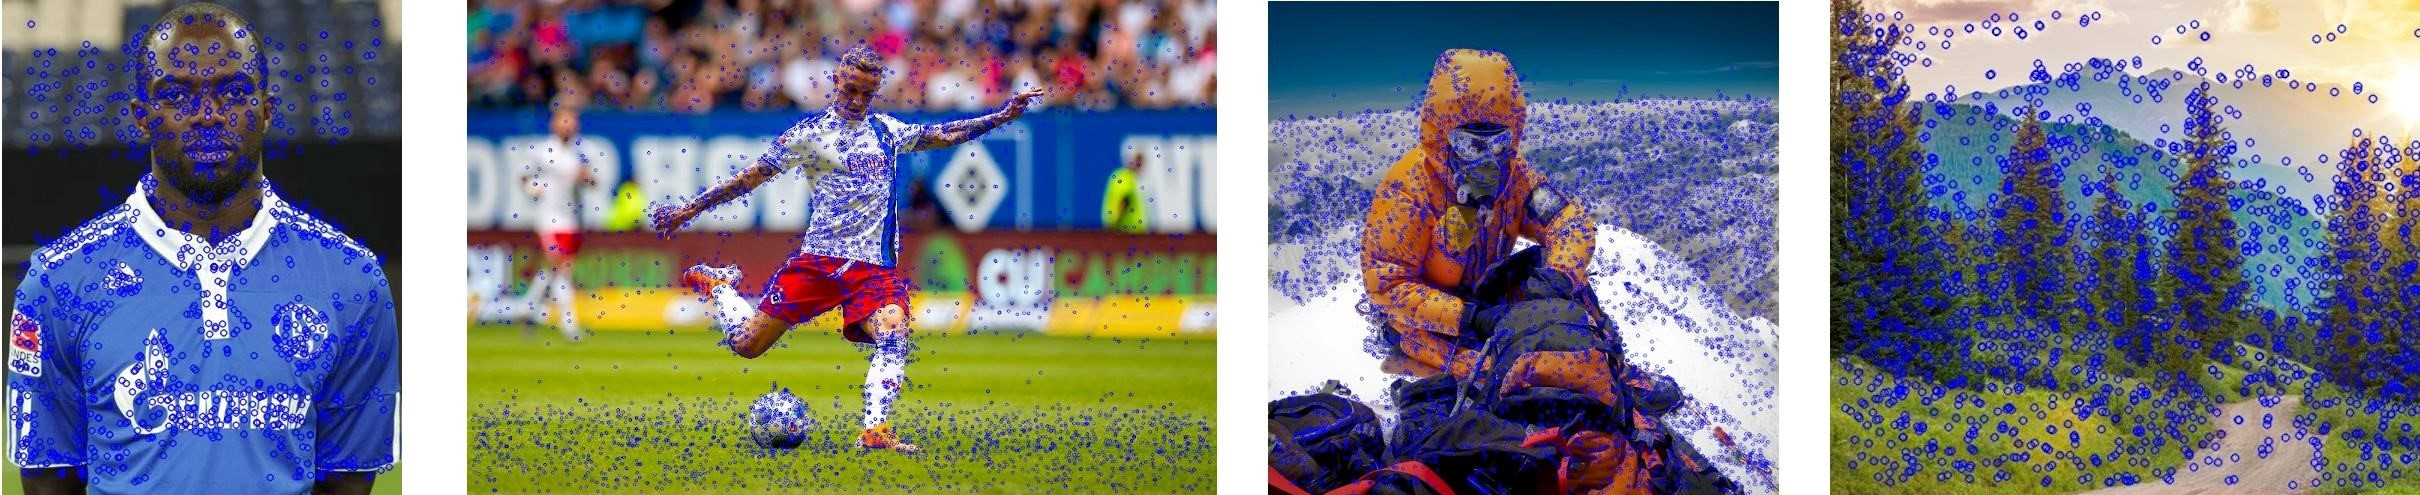
\includegraphics[scale=0.72]{keypoints.jpg}
\label{fig:keypoints}
\caption{Vier Beispielbilder mit blau markierten Keypoints ermittelt durch einen SURF-Detektor}
\end{center}
\end{figure}

\subsection{Keypoint Description}
Für die Keypoints in Bildern können Deskriptoren berechnet werden. Ein Deskriptor hat die Aufgabe einen Keypoint so zu beschreiben, dass eine Identifikation des Keypoints auf anderen Bildern möglich wird, indem die umliegenden Elemente des Keypoints betrachtet werden und aus den zur Verfügung stehenden Informationen ein Vektor berechnet wird. Auch hier soll die Invarianz bei den Keypoints gesichert werden. Mithilfe der in OpenCV enthaltenen Algorithmen zur Berechnung von Deskriptoren wurden zu einem oder mehreren Keypoints jeweils ein Feature-Vektor berechnet, welcher unterschiedliche Informationen über die markanten Bildbereiche, die durch die Keypoints markiert wurden, enthält. Je nach Keypoint-Detektor, der vorher angewandt wurde, konnten wir unterschiedich viele Eigenschaften für gleiche Keypoint Ansammlungen ermitteln. Nach einer Reihe von Tests haben wir uns für den SURF-Detektor entschieden, da dieser im Verhältnis zu den anderen Detektoren die kürzeste Berechnungsdauer hat. Der \textit{Speeded Up Robust Features} Algorithmus erzeugt dabei Features mit 64 Dimensionen bzw. Keypointeigenschaften. 

\subsection{Signaturen}
Da Bilder oftmals tausende von Keypoints beinhalten können, ist ein Vergleich aller Keypoints nicht zielführend. Deshalb wird im Bereich Computer Vision oft mit Signaturen oder Histogrammen gearbeitet. Da wir im späteren Verlauf Distanzen auf Basis der \textit{Earth Mover's Distance} berechnen wollen, haben wir uns in einem frühen Stadium für den Einsatz von Signaturen entschieden. Beim Konzept der Signaturen werden ähnliche Keypoints geclustert und ihre Deskriptoren zu repräsentativen Feature-Vektoren zusammengefasst. Dabei kann jedes Bild unterschiedlich viele Signaturen mit einer unterschiedlichen Anzahl an Keypoints, sogenannten Gewichten, enthalten.
\\
\\
Beliebte Algorithmen zum Clustern von Featuren sind der  \textit{k-Means}-Algorithmus sowie \textit{DBSCAN} (Density-Based Spatial Clustering of Applications with Noise). Beim \textit{k-Means}-Verfahren wird für jedes Bild eine statische Anzahl an $k$ Clustern bestimmt. Da die Anzahl an Clustern in einem Bild Einfluss auf die Qualität der einzelnen Signaturen hat, haben wir uns für den  \textit{DBSCAN}-Algorithmus entschieden. Der  \textit{DBSCAN}-Algorithmus ist ein dichtebasierter Algorithmus, bei dem die Anzahl an Clustern dynamisch bestimmt wird. Dieser basiert auf der Annahme, dass zwei Objekte als \textit{dichte-verbunden} gelten, wenn es eine Kette von \textit{dichten} Objekten gibt, die diese Punkte miteinander verbinden. Die dadurch verbundenen Punkte bilden ein Cluster. Der Algorithmus verfügt über zwei Parameter $\epsilon$ und $minPts$. Dabei definiert $\epsilon$ die maximale Länge, bei der zwei Punkte als Nachbarn gelten, wenn die Distanz zwischen ihnen  $< \epsilon$ ist. Der Parameter $minPts$  bestimmt wann Objekte als \textit{dicht} gelten. Und zwar wenn es mindestens $minPts$ über $\epsilon$ erreichbare Nachbarn gibt.
\\
\\
\begin{figure}[h]
\begin{center}
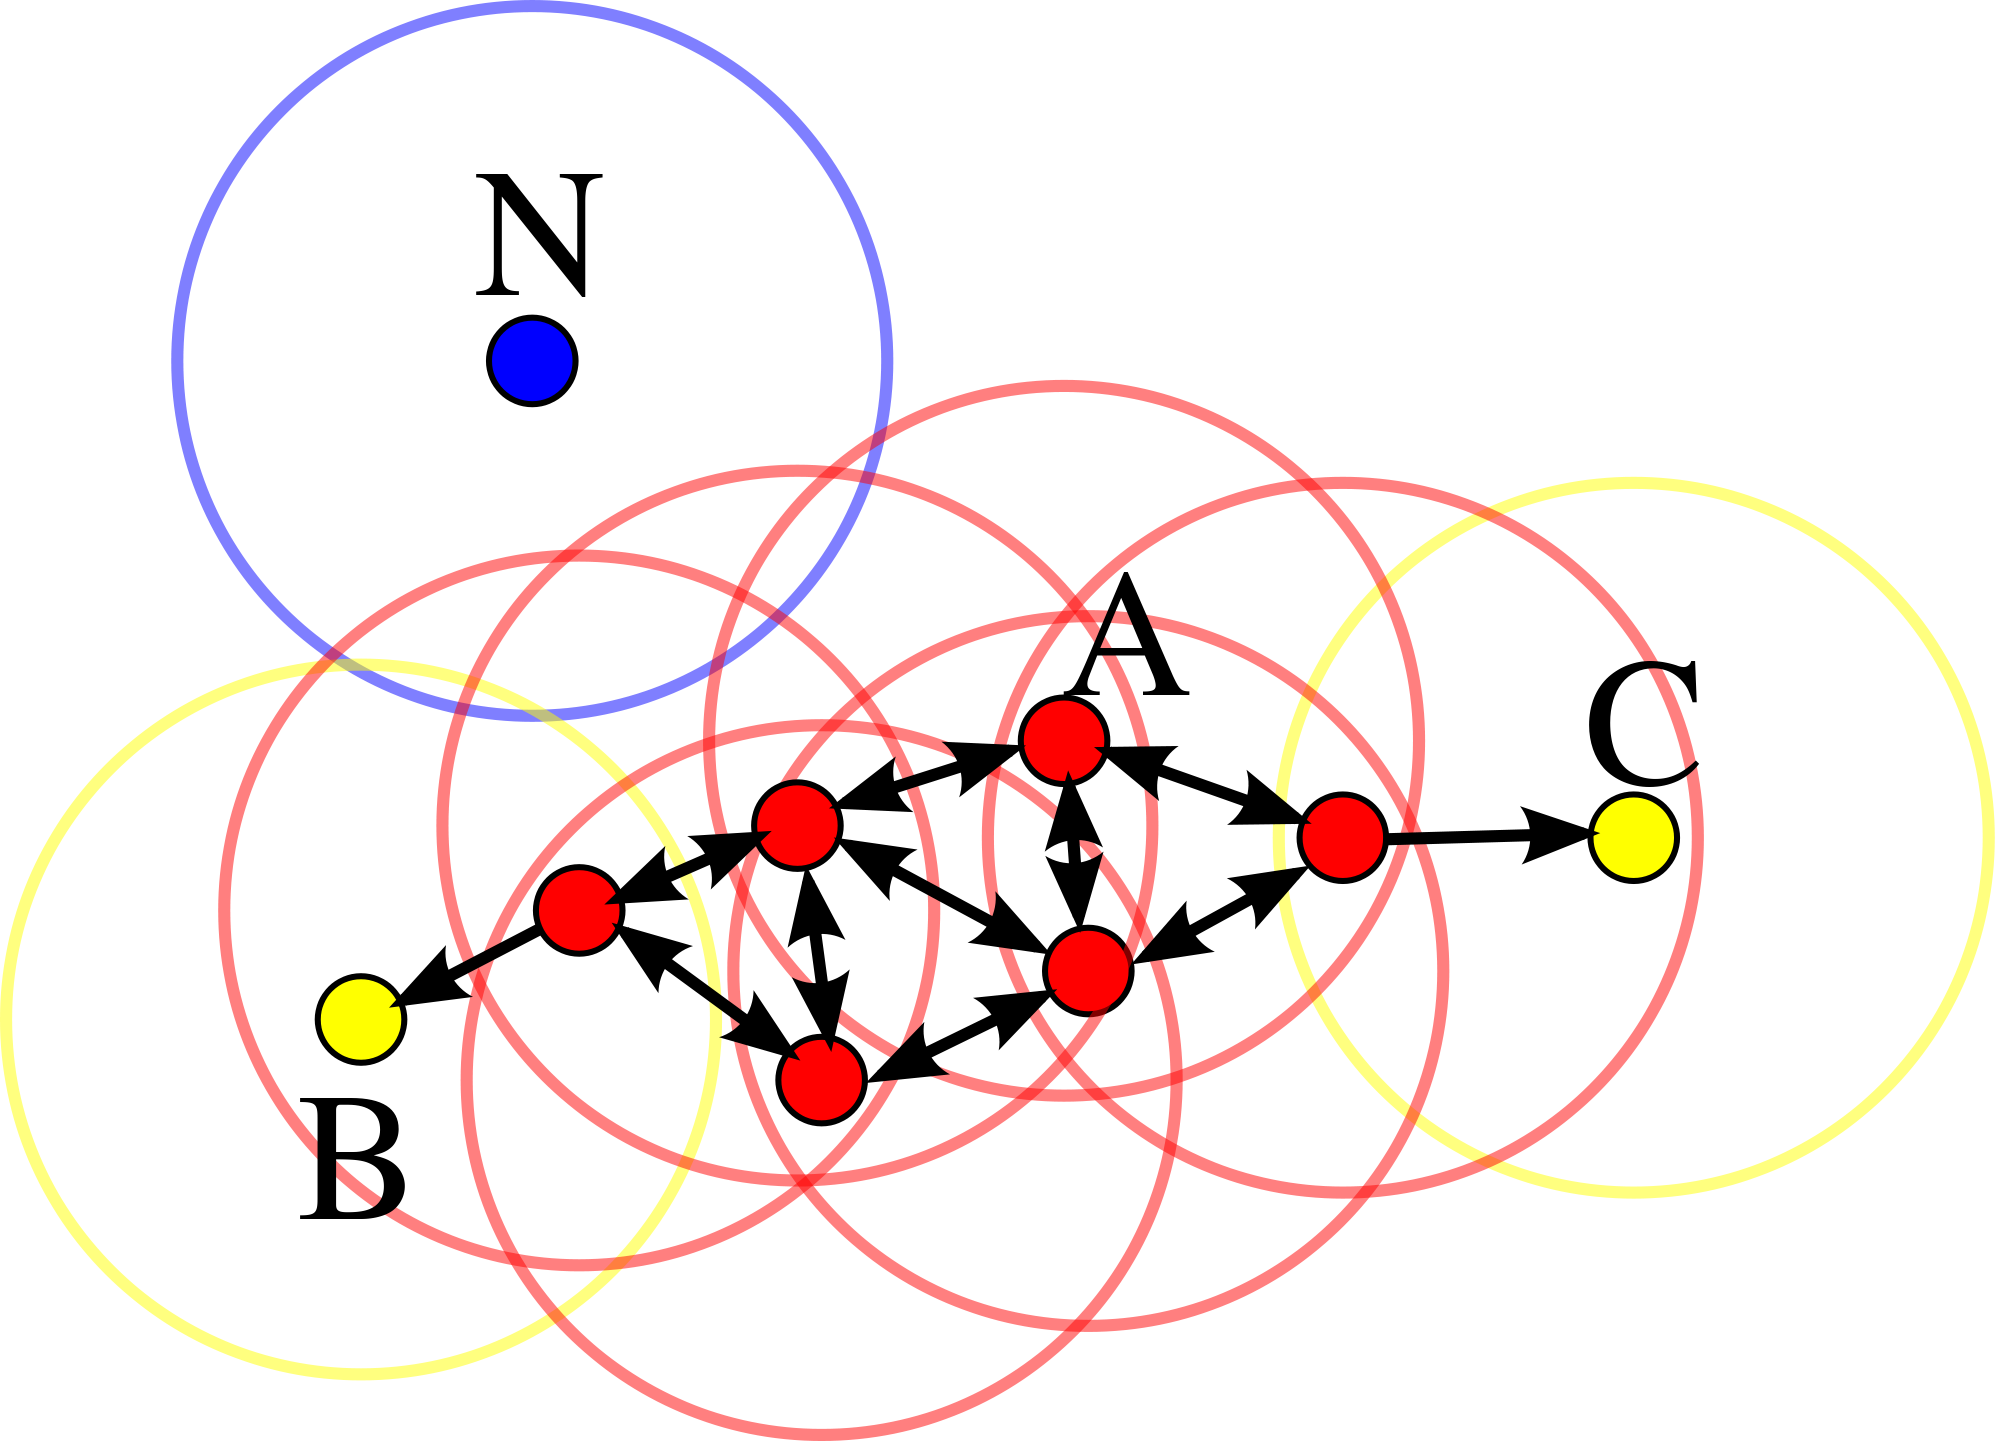
\includegraphics[scale=0.15]{dbscan.png}
\label{fig:DBSCAN}
\caption{DBSCAN-Algorithmus}
\end{center}
\end{figure}
\\
\\
Abbildung 2 visualisiert den Vorgang des Clusterns - Die roten Punkte bei A sind Kernpunkte. Das bedeutet, dass für diese Punkte die Distanz untereinander kleiner als $\epsilon$ ist und mindestens $minPts$ Nachbarn vorhanden sind. Diese bilden dann ein Cluster. Für die Punkte B und C gilt zwar $\epsilon$ zu einem Punkt, jedoch nicht zu $minPts$, sie gehören also gerade noch so zum Cluster und Punkt N erfüllt keine der Eigenschaften, ist also kein Teil des Clusters.  
\\
\\
Bei der Implementierung des DBSCAN-Algorithmus wurde die Klasse \textit{DBSCANClusterer} aus dem Package \textit{org.apache.commons.math3.stat.clustering} von Apache verwendet. Für die Signaturen wird der Mittelwert über jedes Feature der einzelnen Deskriptoren gebildet, welches in das entrpechende Cluster fallen. Dadurch entsteht im Fall von \textit{SURF} ein zentrierten Feature-Vektor mit 64 Dimensionen, der repräsentativ für das gesamte Cluster ist. Zusätzlich wird das Gewicht jeder Signatur gespeichert, damit diese bei der Distanzberechnung miteinfließen können.

\subsection{Ähnlichkeitsmaß}
Auf Basis der zuvor ermittelten Signaturen werden im nächsten Schritt Distanzfunktionen eingeführt um die Ähnlichkeit zwischen Objekten zu messen. Dabei haben wir die \textit{Earth Mover's Distance} mit dem Euklid- sowie Hamming-Distanzmaß näher untersucht. Den ebenfalls implementierten \textit{Jaccard}-Koeffizient zur Distanzberechnung mussten wir für den Test verwerfen, da die Berechnungen und Vergleiche aufgrund der Anzahl an Keypoints in den getesteten Bildern zu komplex wurden.
\\
\\
Zunächst haben wir einen Ansatz gewählt bei welchem wir die Distanzen aller Signaturen zueinander berechnen und mit den zuvor ermittelten Gewichten multiplizieren und dann durch das Gesamtgewicht teilen. Die Distanz zwischen zwei angenommen dreidimensionalen Signaturen würde sich somit wie folgt berechen: 
\\
\\
$d = dist * \frac {24 + 7} {233 + 75} = 0,4026$,
\\
\\
wobei 
\\
\\
$dist = \left( \begin{array}{c} 3 \\ 6 \\ 9 \end{array}\right) - \left( \begin{array}{c} 2 \\ 4 \\ 8 \end{array}\right)$.
\\ 
\\
\\
Dabei hat Signatur $s_{1} = (3,6,9)^{T}$ ein Gewicht von $24$ und Signatur $s_{2} = (2,4,8)^{T}$ ein Gewicht von $7$. Das Bild von Signatur $s_{1}$ hat über alle Signaturen summiert ein Gewicht von 233 und das Bild von Signatur $s_{2}$ ein Gewicht von 75.
\\
\\
Diese Methode brachte uns jedoch unbefriedigende Ergebnisse, da eine solche Distanzfunktion keine wünschenswerten  Eigenschaften aufweist. Beispielsweise kann die Distanz zu einem identischen Bild nie Null sein, wenn mindestens ein Bild mehr als eine Signatur hat. Ebenso ist die Distanzfunktion auch nicht skalierungs- und rotationsinvariant. 
\\
\\ 
Eine etwas anspruchvollere Funktion ist die \textit{Earth Mover's Distance}. Diese löst ein Optimierungsproblem und interpretiert dabei  die Signaturen des einen Bildes als Erdhaufen und die Signaturen des anderen Bildes als Erdlöcher. Ziel ist es dabei die gesamte Erdmasse von $A$ (Gesamtgewicht von Bild $A$) in die Löcher von $B$ (Gesamtgewicht von Bild $B$) zu befördern, wobei die zurückgelegte Gesamtdistanz zwischen $A$ und $B$ minimiert werden soll. Die Gesamtdistanz ergibt sich aus den Distanzen der einzelnen Signaturen von $A$ und $B$ multipliziert mit der Erdmasse (Gewicht von $A$), die auf diesen Strecken befördert wird. Für Löcher oder Erdhaufen, die aufgrund von unterschiedlichen Gesamtgewichten zweier Bilder übrig bleiben, wird ein Strafwert je Einheit zur Gesamtdistanz aufaddiert.
\\
\\
Auch für dieses Problem haben wir eine Klassenbibliothek in Java gefunden, die viele Funktionen der \textit{Earth Mover's Distance} implementiert. Die JAR-Datei \textit{JFastEMD} beinhaltet unter Anderem eine \textit{Signature-}Klasse, an welche wir den zentrierten Feature-Vektor eines unserer Cluster sowie das entsprechende Gewicht übergeben. Das Interface \textit{Feature} definiert die Eigenschaften eines Features innerhalb einer Signatur, wobei es durch die Klasse \textit{Feature2D} implementiert wird. In \textit{Feature2D} wird mit zweidimensionalen Featuren gearbeitet sowie eine Methode zur Berechnung von euklidischen Distanzen mittels der Funktion \textit{groundDist(Feature f)} implementiert. Da wir in unserem Fall mit eindimensionalen Features arbeiten, welche im Vektor vom Typ \textit{double[]} vorliegen, mussten wir die JAR-Datei modifizieren und das Interface \textit{Feature} sowie die Klasse \textit{Feature2D} verändern. Die Klasse \textit{Feature2D} haben wir in \textit{Feature1D} umbennant, wobei wir dort zusätzlich neben der Funktion zur Berechnung der euklidischen Distanz eine Funktion zur Berechnung der Hamming-Distanz implementiert haben. Die Hauptklasse \textit{JFastEMD} berechnet dann schließlich die Earth Mover's Distance mit Hilfe der zuvor genannten Hilfsklassen. Die Methode zur Berechnung der Earth Mover's Distance sieht wie folgt aus:
\\
\\
$double$ $distance(Signature$ $signature1,$ $Signature$  $signature2,$ $double$ $extraMassPenalty)$,
\\
\\
wobei der Paramter \textit{extraMassPenalty} den Strafwert für übrig gebliebene Erde definiert. Bei $-1$ wird je Einheit die höchste Distanz der beiden Signaturen zur Gesamtdistanz aufaddiert. Bei $0$ ist der Strafwert $0$. Alle anderen positiven Werte ergeben fixe Strafwerte.
\\
\\
Der \textit{Jaccard}-Koeffizient hingegen verfolgt einen anderen Ansatz. Dieser wird hauptsächlich als Ähnlichkeitsmaß für Mengen und auch Vektoren verwendet, ist also für unseren Anwendungsfall nicht ganz ungeeignet.
Berechnet wird der Koeffizient $J$ durch eine Divison der Schnittmenge zweier Mengen bzw. Vektoren $A$ und $B$ durch deren Vereinigungsmenge. In der Natur des Ähnlichkeitsmaßes liegt also eine prozentuale Bewertung der Ähnlichkeit zweier Vektoren (oder Deskriptoren). Je höher der Koeffizient ist desto ähnlicher sind sich die Vergleichenen Deskriptoren, damit auch die Keypoints und im Optimalfall der Bildbereich. 
\\
\\
$J(A,B) = \frac {{{A}\cap{B}}}  {{A}\cup{B}}$.
\\
\\
Der Algorithmus ist so implementiert, dass zwischen den zu vergleichenden Bilder die Deskriptoren miteinander verglichen werden. Dabei wird im Vorfeld ein Schwellwert (Threshold) festgelegt, welcher die maximal erlaubte Distanz beschreibt. Ist der Algorithmus jetzt dabei, einen Deskriptor $D1$ aus Bild 1 mit einem Deskriptor $D2$ aus Bild 2 zu vergleichen, so werden die einzelnen Keypoints aus dem Deskriptor $D1$ mit allen Keypoints aus dem Deskriptor $D2$ verglichen. Die Distanzen, die kleiner als der Threshold sind, werden zur Schnittmenge hinzugezählt. Je höher die Schnittmenge, desto höher der Jaccard-Koeffizient und desto höher die Ähnlichkeit der verglichenen Bilder.
\\
\\
Vergleicht man als Beispiel nun zwei Bilder miteinander, die 200 und 300 Deskriptoren haben, so müssten $200 \cdot 300=6000$ Vergleiche ausgeführt werden. Bei 64 Dimensionen pro Deskriptor wären das $6000 \cdot 64 = 384000$ Berechnungen für den Vergleich zweier Bilder. Durch den hohen Berechnungsaufwand haben wir uns auf die \textit{Earth Mover's Distance} beschränkt.


\subsection{Anfrageform und Indexierung}
Die zu vergleichenden Bilder, werden als Menge in Form eines Ordners in der UI unseres Programmes ausgewählt. Zuvor muss das so genannte Input Image ausgewählt werden mit dem die Menge an Bildern verglichen wird. In der UI können die Parameter: $minSamples$, $eps$, $EMD Penalty$ vor jedem Durchlauf angepasst werden. Als Algorithmus kann entweder der EMD Algorithmus mit Hamming Distanz oder mit euklidischer Distanz ausgewählt werden. Die verglichenen Bilder werden anschließend nach ihrer Distanz zum Input Image sortiert und in einem neuen Ordner gespeichert. In diesem Ordner befindet sich ebenfalls eine Textdatei, die einen Score (siehe Abschnitt 3.2) berechnet sowie die Berechnungsdauer des jeweiligen Durchlaufs dokumentiert.

\subsection{Schlussfolgerung}
Die Implementierung der einzelnen Distanzalgorithmen sowie der Keypointdetection gestaltete sich als wesentlich aufwendiger als gedacht. Dies ist zurückzuführen auf unzureichende Kompatibilität im Rahmen der Funktionalitäten der bereits in der Literatur/ im Internet vorhandenen Algorithmen. Diese mussten durch uns kontinuierlich angepasst oder neu geschrieben werden. Ebenfalls stellten wir fest, dass sich Dateiformate von Bildern (png, jpg, ...) in ihrer Struktur grundlegend unterscheiden können und sich dadurch die Nutzung verschiedener Bilder beziehungsweise deren Vereinbarkeit mit genutzten Algorithmen schwierig gestaltete. 

\section{Durchführung}
Wie bereits beschrieben, mussten wir uns aufgrund des enormen Rechenaufwands für den Jaccard-Koeffizienten auf den EDM-Algorithmus beschränken. Aufgrund verschiedener Schwierigkeiten bei der Kompatibilität der Bilder und der integrierten Bibliotheken, wurden am Ende insgesamt 8 Durchläufe in die Bewertung aufgenommen. Die Parameter der Durchläufe variieren marginal, die Ergebnisse wiesen jedoch signifikante Unterschiede auf. Davon wurden 4 mit der Hamming-Distanz und 4 mit der euklidischen Distanz durchgeführt, jeweils ein Durchlauf mit verschiedenen Distanzen wiesen die gleichen Parameter auf.
\\
\\
Die getestete Datenbank bestand aus insgesamt 241 Bildern, welche in 7 verschiedene Kategorien unterteilt wurden. Diese Kategorien sind: Autos, Motorrad, Landschaft, Mensch, Pferd, Rad und Schaf. Ausgehend von 10 Testbildern pro Kategorie, wurden für jedes getestete Bild drei Transformationen durchgeführt um die verschiedenen Eigenschaften des Keypointdetectors SURF sowie des EDM-Algorithmus auf deren Robustheit zu prüfen. 

\subsection{Transformationen}
Der SURF-Algorithmus zur Keypointdetection weist verschiedene Eigenschaften auf, die die Robustheit des Algorithmus definieren. Dazu gehören die Skalierungs-, Rotations- und Belichtungsinvarianz. Da die Skalierungsinvarianz nicht durch eine einfache Transformation getestet werden kann, beschränkten wir uns auf die Rotations- und Belichtungsinvarianz. Dafür wurde jedes der Testbilder aus der Datenbank einmal um 90 Grad rotiert, gespiegelt und in Graustufen umgewandelt. Pro Testbild ergaben sich somit insgesamt 4 zu vergleichende Bilder. Mit 10 Bildern pro Kategorie ergaben sich in Theorie somit insgesamt 40 Bilder pro Kategorie. Da einige der Bilder trotz ihres passenden Formats nicht verglichen werden konnten und sich durch die Transformationen teilweise Komplikationen ergaben, konnten einige der Bilder nicht in die Berechnungen aufgenommen werden.

\subsection{Scores}
Zur Evaluierung haben wir insgesamt vier Variablen zur Bewertung hinzugezogen. Dazu gehören der Gesamtscore eines Bildes sowie drei separate Scores zu den Transformationen der einzelnen Bilder.

\subsubsection{Gesamtscore}
Der Gesamtscore wird pro Bild berechnet und setzt sich wie folgt zusammen: Zu Beginn ist der Gesamtscore des Bildes 0. Nachdem das Referenzbild mit allen anderen aus der Datenbank verglichen wurde, wird ein Ranking vollzogen. Dabei werden alle anderen Bilder aus der Datenbank entsprechend ihren Gesamtdistanzen zum Referenzbild aufsteigend sortiert. Das Bild an erster Stelle hat die kleinste Distanz zum Referenzbild, das Bild an zweiter stelle die zweitkleinste Distanz usw. Nun werden die ersten zehn Bilder aus der Liste bewertet. Ist das verglichene Bild eine Transformation des Originalbildes (z.B. Referenzbild $Auto01$ und $Auto01\_mir$ ist unter den ersten zehn Bildern) erhöht sich der Score um zwei. Ist ein Bild aus der gleichen Kategorie (z.B. Referenzbild $Auto01$ und $Auto02$ ist unter den ersten zehn Bildern) erhöht sich der Score um 1. Ist das Vergleichsbild nicht aus derselben Kategorie (z.B. Referenzbild $Auto01$ und $Pferd01$ ist unter den ersten zehn Bildern) gibt es keinen Punkt.
Je mehr Bilder aus derselben Kategorie also unter den ersten zehn Bildern sind, desto höher ist der Score und desto genauer ist der Algorithmus.

\subsubsection{Score BW, MIR, ROT}
Score BW gibt den Score für die Bilder an, die in Graustufen transformiert wurden. Anders als beim Gesamtscore ist hier das Ranking für das transformierte Bild relevanter. Je höher das in Graustufen transformierte Bild platziert ist, desto höher fällt Score BW aus. Ist z.B. $Auto03$ das Referenzbild und $Auto03\_bw$ auf Platz 2, so wird Score BW um 10-1 (da 10 Plätze und bei 0 beginnend), also 9 erhöht. Ist $Auto03\_bw$ auf Platz 8, so wären es 10-7, also 3 Punkte. Die Scores der anderen Transformationen ergeben sich analog.

\subsection{Robustheit}
Die Robustheit der Keypointdetection und des EMD-Algorithmus haben wir durch den Vergleich der Leistung innerhalb und übergreifend der Bildkategorien abgebildet. Dadurch können wir ebenfalls Aussagen dazu treffen, mit welcher Art von Kategorie die Algorithmen besonders gut funktionieren. Um also die Robustheit zu prüfen, haben wir die kumulierten und durchschnittlichen Distanzen für Bildvergleiche pro Kategorie zusammengezählt und Ausreißer identifiziert. Als Referenzwert für eine Kategorie, z.B. $Auto$, haben wir die durchschnittliche Distanz der Bilder in der Kategorie $Auto$ untereinander berechnet. D.h. insgesamt 10 Referenzwerte ($Auto01$ zu allen Autobildern, $Auto02$ zu allen Autobildern, ...). Anschließend haben wir für jeden Vergleich die durchschnittliche Distanz zu anderen Kategorien berechnet um im Anschluss die Abweichung von der Referenzdistanz zu betrachten.
Beispiel: Die durchschnittliche Distanz von $Auto01$ zu allen Autobildern beträgt 500 und stellt die Referenzdistanz dar. Nun werden die durchschnittlichen Distanzen von $Auto01$ zu allen Bildern der anderen Kategorien berechnet. Für diese Ergeben sich z.B.: $Auto01$ zu Motorrad = 750, zu Landschaft = 860, zu Mensch = 450, zu Pferd = 1500, zu Rad = 780 und zu Schaf = 210. Die Kategorien Mensch und Schaf weisen eine geringere Durchschnittsdistanz zu Auto auf als Auto zu sich selbst. Hier können dann zwei Ausreißer festgestellt werden.Ab mehr als 50\% bei der Anzahl der Kategorien, also vier, ist die Abweichung kritisch zu betrachten. Um eine genauere Aussage treffen zu können, wird das ganze nun mit $Auto02$, $Auto03$ etc. durchgeführt und die Ausreißer kumuliert. Je mehr Ausreißer eine Kategorie besitzt, desto unpräziser ist die Kombination aus SURF und EMD für entsprechende Kategorie.

\section{Ergebnisse}
Test von verschiedenen Distanzfunktionen (Jaccard, EMD), verschiedern Penalty-Werte für EMD sowie Verwendung Distanzmaße (euklidisch, Hamming). Eventuell verschiedene Parameter bei DBSCAN-Clustering testen.


\subsection{Earth Mover's Distance}

\subsection{Jaccard-Koeffizient}

\subsection{Schlussfolgerung}

\FloatBarrier

\section{Ausblick}

\section{Arbeitsaufteilung}

\end{document}
